\subsection{Red corporativa mediana}

Esta es una red de la cuál conocemos la topología: consiste de un único router al cuál se conectan unas 30 pc's y una cantidad similar de celulares.


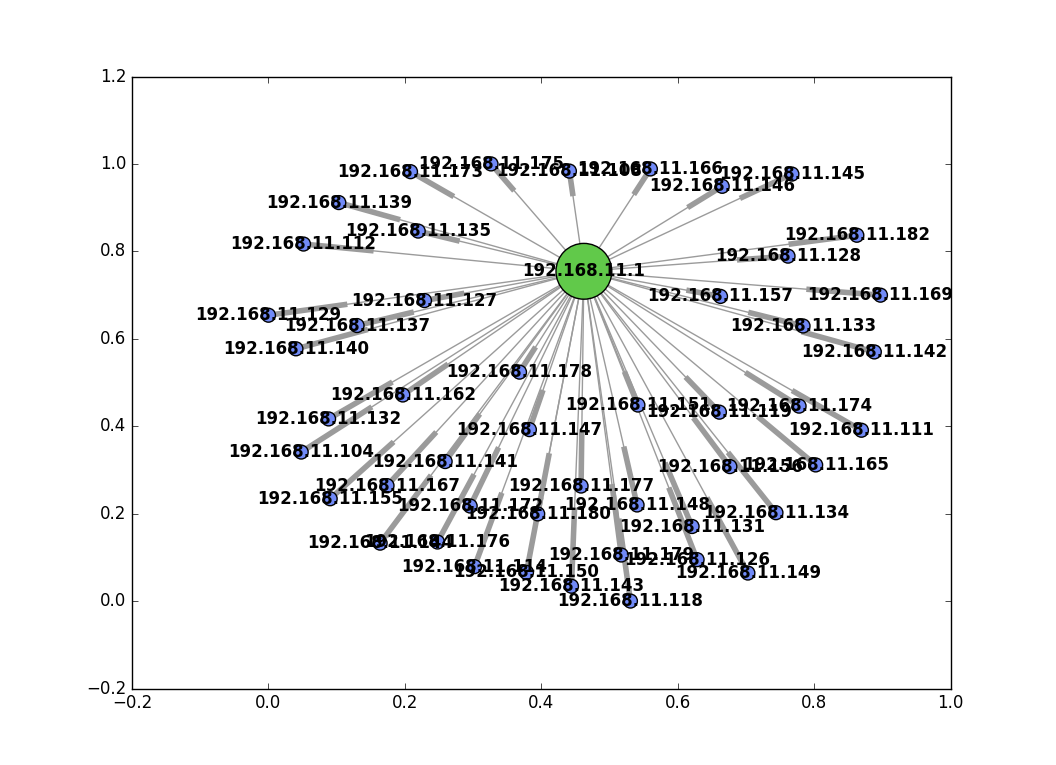
\includegraphics[scale=0.65]{imagenes/captura-red-trabajo-grafo.png}

Se puede ver que el default gateway (192.168.11.1), aparece como el nodo central al cual todo el resto de los nodos se conectan.

A continuación mostramos la entropía de las fuentes $S$ y $S1$ y la información de cada símbolo:

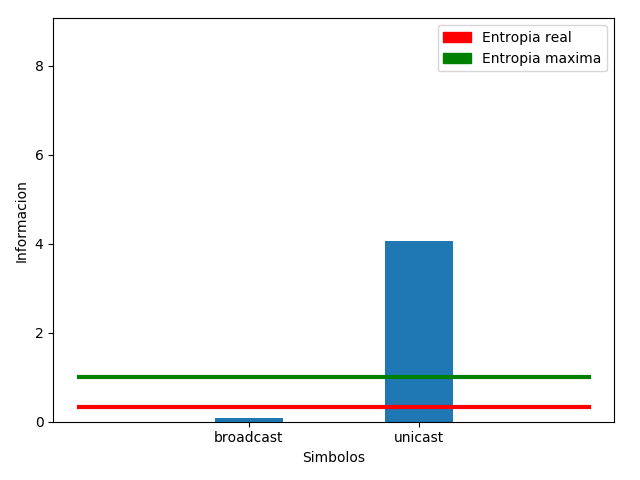
\includegraphics[scale=0.65]{imagenes/captura-red-trabajo-fuente-s.png}

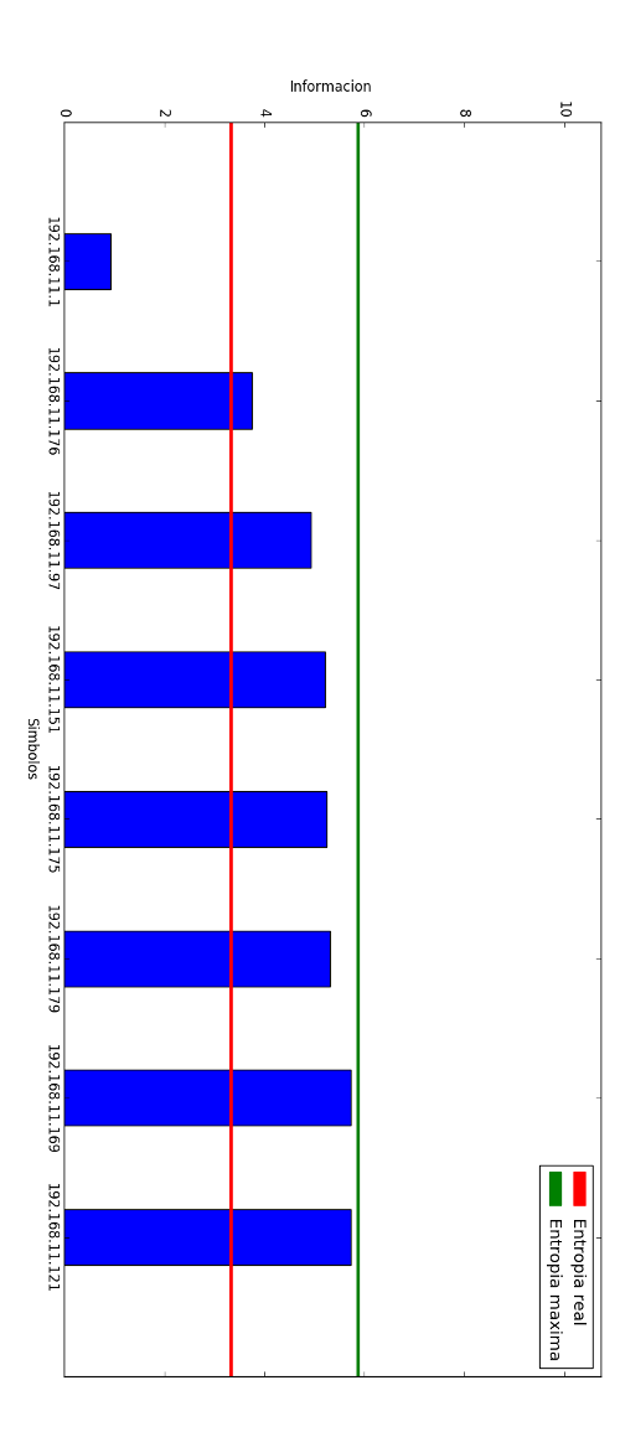
\includegraphics[scale=0.65]{imagenes/captura-red-trabajo-fuente-s1.png}

Tanto para $S$ como para $S1$ podemos observar que la entropía es menor que la entropía máxima. Sabemos que una fuente de memoria nula tiene entropía máxima cuando todos sus símbolos son equiprobables. Que la entropía real sea menor nos indica que hay ciertos símbolos más probables que otros. 

En el caso de la fuente $S$, en la captura observamos que el router está constantemente emitiendo paquetes \textit{Who-has}. Por lo tanto, observar el símbolo \textit{Broadcast} es altamente probable, lo cual implica que aporta muy poca información (0.0894 bits), mientras que el símbolo \textit{Unicast} aporta mucha más información (4.0557 bits), haciendo que \textit{Broadcast} sea un nodo distinguido, ya que la entropía de la fuente es 0.3279. La entropía máxima es 10.6995. Creemos que debido a que las tablas de ARP se deben refrescar cada cierto tiempo, la red experimenta un flujo mucho mayor de paquetes \textit{Broadcast} que \textit{Unicast}, dando lugar a una disparidad en la probabilidad de cada símbolo.

En el caso de la fuente $S1$, el único nodo distinguido que nos quedó fue el Default Gateway (pudimos comprobar empíricamente que este nodo lo era ejecutando el comando netstat -nr | grep default), indicando que la manera de seleccionar los símbolos que elegimos para esta fuente funciona muy bien con esta red. Al ser una red con una topología relativamente simple, no podemos asegurar que estos resultados se puedan extrapolar a redes más complejas. Algunos de los otros nodos, como 192.168.11.97 y 192.168.11.151, corresponden a otras notebooks conectadas a la red, lo cual nos resultó un comportamiento extraño. Suponemos que en esas notebooks se estaba ejecutando algún programa que trabaja a bajo nivel y está constantemente obteniendo información de la red local.
